Chapter 11 asked \emph{how much} data. There's a subtler question that
often matters more: what \emph{kind} of data. Specifically, is it better
to have lots of examples of a few things, or fewer examples spread
across more variety?

The easy answer is to treat ``more data'' as one lever. It isn't. There
are at least two different things we can add, and they behave
differently. Think of it like teaching a kid shapes. Show them a hundred
triangles and they'll recognize triangles. Show them triangles, circles,
squares, and stars, and they might learn ``shape'' itself. Same number
of examples, very different kind of learning.

\begin{itemize}
\tightlist
\item
  \textbf{more examples} --- more instances of the same templates, and
\item
  \textbf{more diversity} --- more distinct \emph{kinds} of structure
  and wording.
\end{itemize}

The distinction is important enough to state as a rule:

\begin{quote}
\textbf{More data ≠ more information ≠ more diversity.}
\end{quote}

And this is the chapter where we stop treating it as a hunch and measure
it directly. Because there is a clean way to isolate diversity: hold the
\emph{count} fixed and vary only the \emph{spread}. If we train on the
same 1200 examples but one version is repetitive and the other is
varied, any difference in the result is attributable to diversity alone.

\section{What our experiments hinted}\label{what-our-experiments-hinted}

\begin{figure}
\centering
\pandocbounded{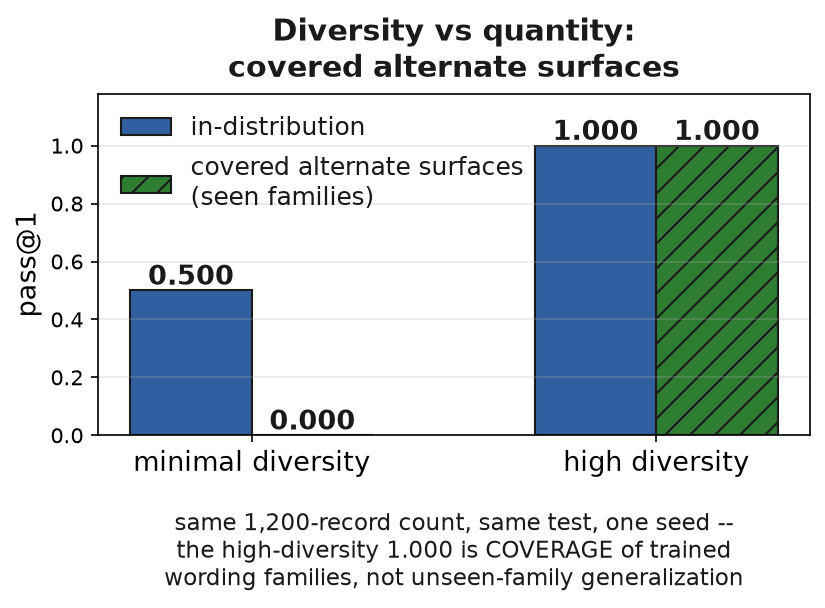
\includegraphics[keepaspectratio,alt={Diversity vs quantity},width=\maxwidth{\textwidth},keepaspectratio]{figures/fig_diversity.png}}
\caption{Diversity vs quantity}
\end{figure}

The data-scaling curve (Chapter 11) showed that simply adding
\emph{examples} of the same sort climbs in-distribution performance ---
0.10 at 100, 0.64 at 3000. So more examples clearly helped the model fit
the pilot task better.

But the \emph{surface} experiment (Chapter 15) exposed the limit of
that: the model's capability collapsed the moment we changed to a
wording it hadn't seen. That is precisely the signature of a model that
was fed \emph{many examples of the same narrow kind} rather than
\emph{diverse kinds}. It learned the particular phrasings well because
it saw many of them, and it learned nothing general because the
diversity was low.

In other words, the very quantity that produced the impressive
in-distribution score is what made it surface-fragile. The model was
well-fed but narrow.

\section{The direct test: same count, different
diversity}\label{the-direct-test-same-count-different-diversity}

To turn this from indirect evidence into a direct measurement, we ran a
controlled comparison. We kept the example count \textbf{identical} ---
the same 1200 examples --- across two training sets:

\begin{itemize}
\tightlist
\item
  \textbf{minimal diversity:} the examples are drawn from a few
  templates with little variation in wording or identifier names.
\item
  \textbf{high diversity:} the same 1200 examples, but spread across
  many phrasings and identifier choices.
\end{itemize}

Because the count is identical, any difference in the result is caused
\emph{only} by the diversity. This is a clean one-variable experiment,
and it is the strongest test of the hypothesis.

\section{The measured result}\label{the-measured-result}

Here is what came out. This is, in our view, the single most actionable
number in the whole book.

\begin{longtable}[]{@{}lll@{}}
\toprule\noalign{}
Training set & in-distribution & surface \\
\midrule\noalign{}
\endhead
\bottomrule\noalign{}
\endlastfoot
\textbf{minimal diversity} & 0.500 & \textbf{0.000} \\
\textbf{high diversity} & \textbf{1.000} & \textbf{1.000} \\
\end{longtable}

Let us read this carefully. Same number of examples --- 1200 in both
cases. But the two models behaved completely differently.

\begin{itemize}
\tightlist
\item
  \textbf{Minimal diversity:} in-distribution 0.500, surface 0.000. The
  model did okay on the narrow task (0.500) but was completely brittle
  to any surface change (0.000). It learned the few phrasings it was
  given and nothing about the \emph{idea}.
\item
  \textbf{High diversity:} in-distribution \textbf{1.000}, surface
  \textbf{1.000}. The model mastered the task \emph{and} held up
  perfectly under surface change. It learned the actual operation, not a
  phrasing.
\end{itemize}

That is a swing from 0.500/0.000 to 1.000/1.000 --- all from changing
\emph{how} the examples varied, not \emph{how many} there were. The same
count. The same model. Only the diversity differed.

\section{What this really means}\label{what-this-really-means}

This is the book's most useful finding, and it reframes the whole data
question. It is not that ``more data is better.'' It is that \textbf{the
kind of variation in the data is what creates robust capability.}

A model fed many examples of few phrasings memorizes the phrasings. A
model fed the same number of examples spread across many phrasings
learns the \emph{underlying operation} --- because the only thing that
stays constant across varied phrasings is the operation itself. When the
wording varies but the meaning stays the same, the model has no choice
but to attach its learning to the meaning rather than to any particular
surface. Diversity does not just add information; it \emph{forces}
abstraction.

This connects directly to the book's central theme. We spent the book
asking whether the model \emph{learned} or merely associated. Here is a
lever that pushes it from association toward learning: vary the surface
form until the only stable thing is the meaning. The model's inability
to generalize under repetition was not a mysterious limitation --- it
was a direct consequence of a training set that gave it no reason to
abstract.

\section{The honest caveat}\label{the-honest-caveat}

It is worth noting that this experiment measured \emph{surface}
diversity. It showed that varying phrasing and identifiers makes the
model robust to surface change (the Level-3 boundary). It does
\textbf{not} show that diversity fixes \emph{compositional}
generalization (the Level-4 boundary) --- that is a separate, harder
question. Whether the same lever helps a model combine two things it
knows is the most natural next experiment, and it is called out in the
conclusion.

So the honest scope of the finding is precise: \textbf{diversity ---
specifically surface variance --- is what creates surface robustness,
far more than the sheer number of examples does.} Whether diversity
reaches deeper, into composition, remains open.

\section{The lesson}\label{the-lesson}

This reframes what ``more data'' buys. To make a capability
\emph{robust}, we need not just more examples of a phrasing, but more
\emph{diverse} phrasings, identifiers, and structures --- enough that
the model cannot tie the operation to any particular surface form. Our
experiments show the model's weakness is not a lack of data
\emph{quantity}, but a lack of data \emph{diversity} (and, deeper, a
lack of the structural kind of data needed for composition --- see
Chapter 16).

The practical implication is genuinely surprising and useful: a
practitioner who cannot acquire more data can often get a large
improvement just by \emph{diversifying} the data they already have.
Re-phrasing the same examples, varying the identifiers, and spreading
across template families can turn a brittle 0.500/0.000 model into a
robust 1.000/1.000 --- with zero additional data. That is the kind of
result that changes how a dataset would actually be built.
